%!TEX root = ../template.tex
%%%%%%%%%%%%%%%%%%%%%%%%%%%%%%%%%%%%%%%%%%%%%%%%%%%%%%%%%%%%%%%%%%%%
%% appendix1.tex
%% NOVA thesis document file
%%
%% Chapter with example of appendix with a short dummy text
%%%%%%%%%%%%%%%%%%%%%%%%%%%%%%%%%%%%%%%%%%%%%%%%%%%%%%%%%%%%%%%%%%%%

\typeout{NT FILE appendix1.tex}%

\chapter{Additional Simulation Studies}
\label{app:rpc_plots}


%This appendix presents additional figures from the simulation studies performed prior to the experiment. While the main discussion in Chapter \ref{cha:simulations} focused on the most relevant results for the interpretation of the experiment and the training of the multidimensional fitting (MDF) functions, the plots shown here provide complementary information regarding the expected fragment composition and detector response.  

%The purpose of including these results is to give a broader view of the simulated conditions, which can be useful for cross-checks and for future studies within the R$^3$B collaboration. Each figure is accompanied by a short description highlighting its relevance.  

%\begin{figure}[htbp]
%	\centering
%	\begin{minipage}[b]{0.48\textwidth}
%		\centering
%		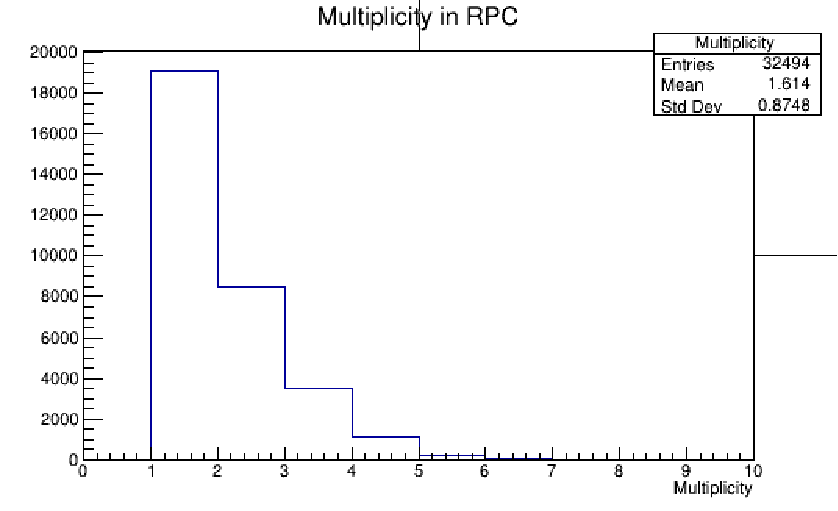
\includegraphics[width=\textwidth]{Appendix/RPCMultiplicity}
%		\caption{Caption for the first figure.}
%	\end{minipage}\hfill
%	\begin{minipage}[b]{0.48\textwidth}
%		\centering
%		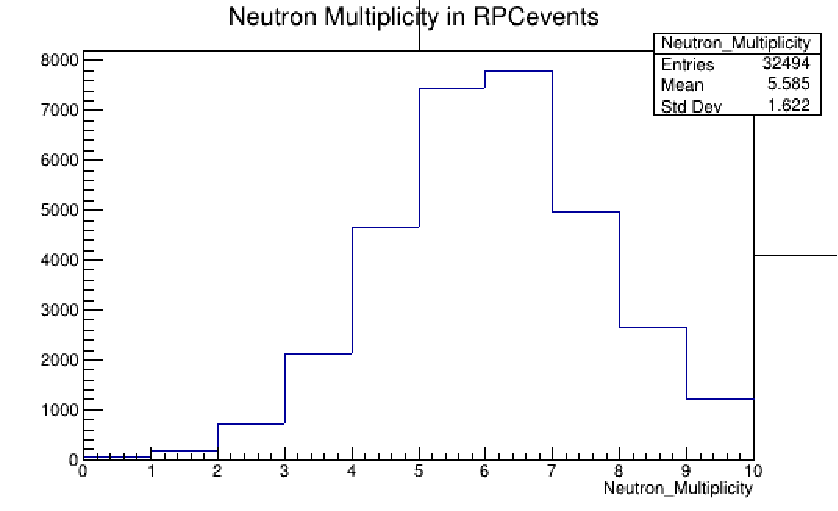
\includegraphics[width=\textwidth]{Appendix/NeutronMulti}
%		\caption{Caption for the second figure.}
%		\label{fig:second}
%	\end{minipage}
%\end{figure}

%\chapter*{Appendix A: Additional Simulation Studies}
%\addcontentsline{toc}{chapter}{Appendix A: Additional Simulation Studies}

This appendix presents additional plots obtained from the simulation studies conducted prior to the experiment. While Chapter \ref{cha:simulations} focused on the main results directly relevant for the positioning of the \gls{RPC} and the development of the multidimensional fitting (\gls{MDF}) functions, the figures shown here provide complementary information on the expected reaction products and the performance of the \gls{RPC}. Each plot is briefly discussed to highlight its relevance and the conclusions that can be drawn.

\section{Multiplicity Distributions}

The first aspect examined in the simulations is the event multiplicity, both in the \gls{RPC} and in the emitted neutrons. These observables provide a global view of the reaction environment that the detectors are expected to face.

\begin{figure}[htbp]
	\centering
	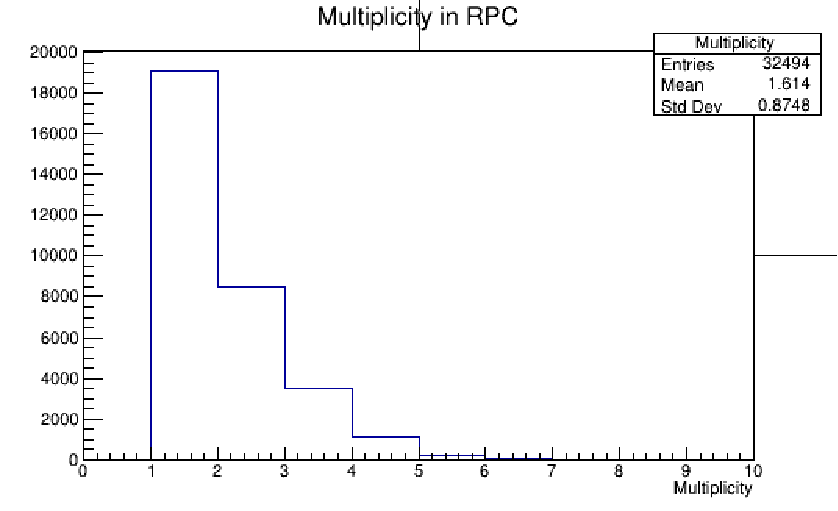
\includegraphics[width=0.7\textwidth]{Appendix/RPCMultiplicity}
	\caption[RPC hit multiplicity distribution]{Distribution of \gls{RPC} hit multiplicities. The most common case corresponds to multiplicity~1, which is favorable as it simplifies the reconstruction. Multiplicity~2 events also occur with non-negligible probability, but they are typically manageable within the \gls{RPC}. Events with higher multiplicities are rare and thus not expected to play a significant role.}
	\label{fig:rpc_multiplicity}
\end{figure}

\begin{figure}[htbp]
	\centering
	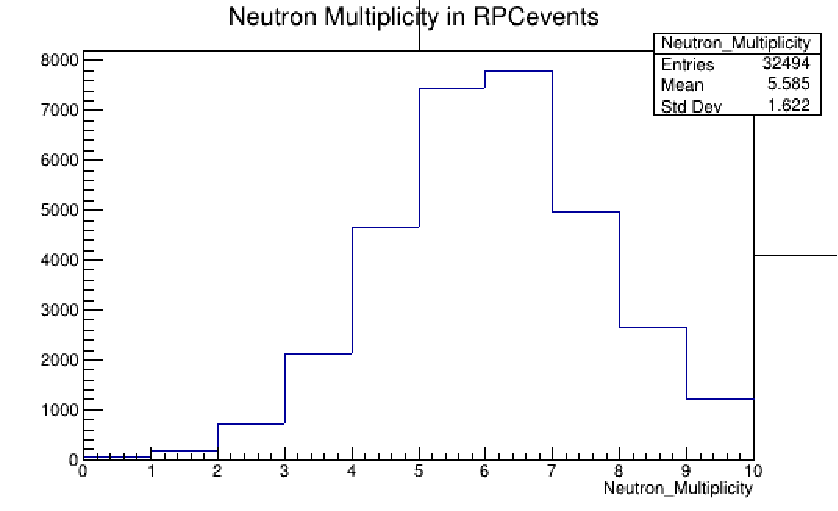
\includegraphics[width=0.7\textwidth]{Appendix/NeutronMulti}
	\caption[Neutron multiplicity distribution]{Distribution of neutron multiplicities from the simulated reactions. The results indicate very high neutron multiplicities, many of which are beyond the resolution capabilities of NeuLAND. As a consequence, a substantial fraction of events will not be fully reconstructable, since part of the neutron information is lost or spread across CALIFA.}
	\label{fig:neutron_multiplicity}
\end{figure}

\section{Fragment Correlations and Channels of Interest}

Beyond multiplicities, the simulations were used to explore correlations between fragments and to identify reaction channels of potential interest.  

\begin{figure}[htbp]
	\centering
	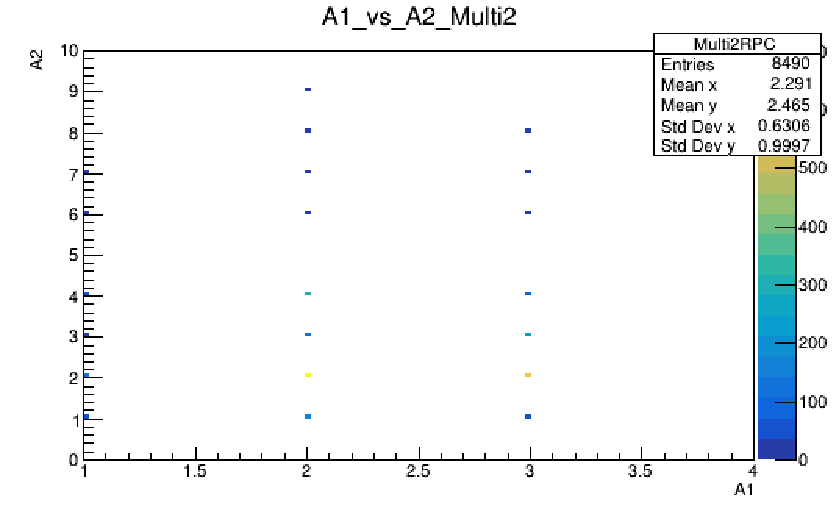
\includegraphics[width=0.7\textwidth]{Appendix/A1vsA2_Multi2}
	\caption[Correlation of fragment masses in RPC multiplicity-2 events]{Correlation between the mass numbers of two fragments reaching the \gls{RPC} in multiplicity~2 events. This plot provides insight into the types of fragment pairs that dominate in such cases, which is useful for evaluating the \gls{RPC}’s reconstruction capabilities when handling multi-hit events.}
	\label{fig:a1_a2}
\end{figure}

\begin{figure}[htbp]
	\centering
	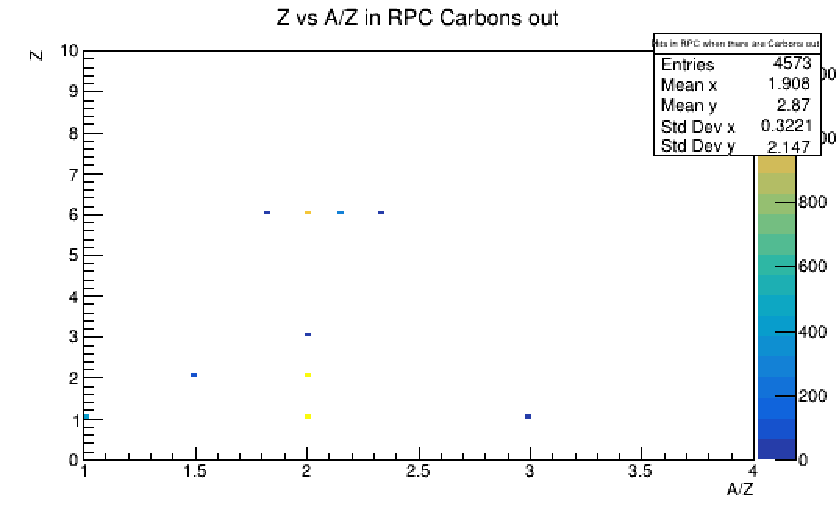
\includegraphics[width=0.7\textwidth]{Appendix/RPCinCout}
	\caption[PID of RPC fragments in events with Carbon residues]{Particle identification (PID) plot of $A/Q$ versus $Q$ in the \gls{RPC} for events where a Carbon residue is produced. This case is of interest since one of the main fragments at the \gls{RPC} are $\alpha$ particles, and the (p,p$\alpha$) channel leading to Carbon is a promising physics case. Studying Carbon residues instead of $\alpha$ particles directly avoids contamination from complete disintegration channels dominated by light fragments (deuterons, tritons, and alphas).}
	\label{fig:pid_carbon}
\end{figure}

\begin{figure}[htbp]
	\centering
	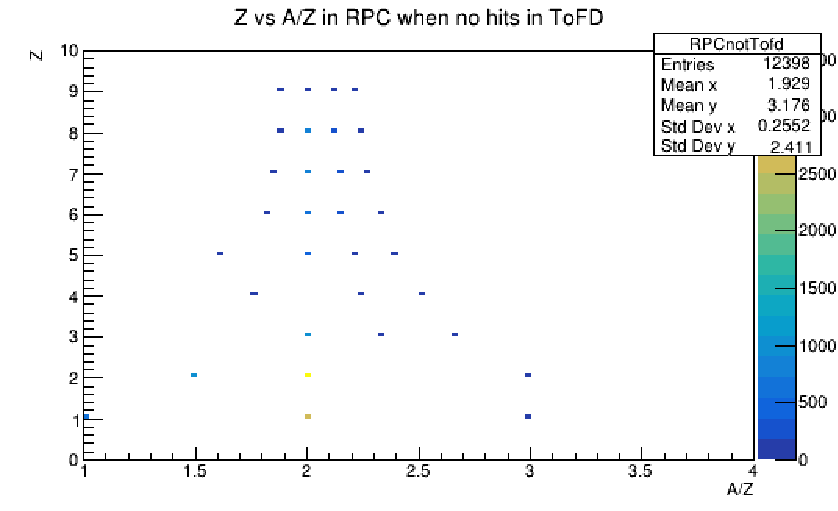
\includegraphics[width=0.7\textwidth]{Appendix/RPCnotTofd}
	\caption[PID of RPC fragments with no ToFD hits]{PID plot ($A/Q$ versus $Q$) for \gls{RPC} fragments in events without a hit in \gls{ToFD}. This scenario is of particular interest, as the veto condition on \gls{ToFD} was later adopted in the real data analysis for the \gls{MDF} application. The plot illustrates the expected distribution under this condition.}
	\label{fig:pid_noToFD}
\end{figure}

\section{Acceptance of the RPC for $A/Q=2$ Fragments}

Since $A/Q=2$ fragments are by far the most abundant species expected at the \gls{RPC}, it is essential to assess the detector’s geometrical acceptance for these particles.  

\begin{figure}[htbp]
	\centering
	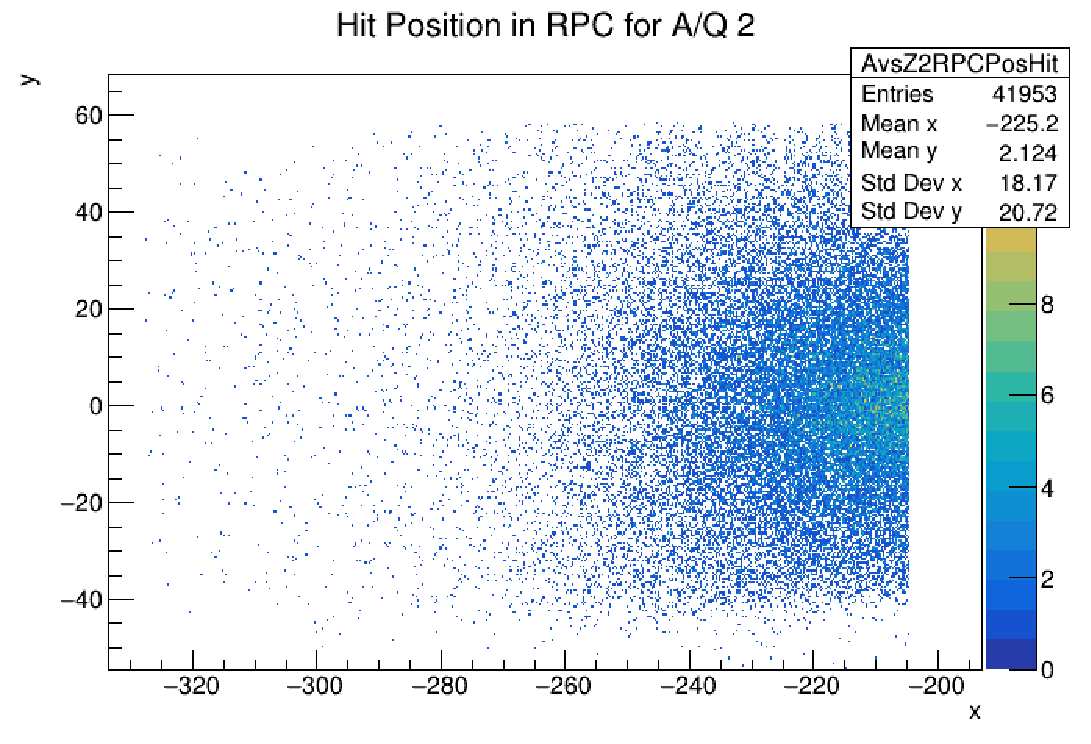
\includegraphics[width=0.7\textwidth]{Appendix/AvsZ2HitPosRPC}
	\caption[RPC hit map for $A/Q=2$ fragments]{Hit map of \gls{RPC} signals for $A/Q=2$ fragments. This case corresponds to the most common species expected at the \gls{RPC}, and the figure provides an overview of the detector’s acceptance for this population.}
	\label{fig:rpc_hitmap_aq2}
\end{figure}

\begin{figure}[htbp]
	\centering
	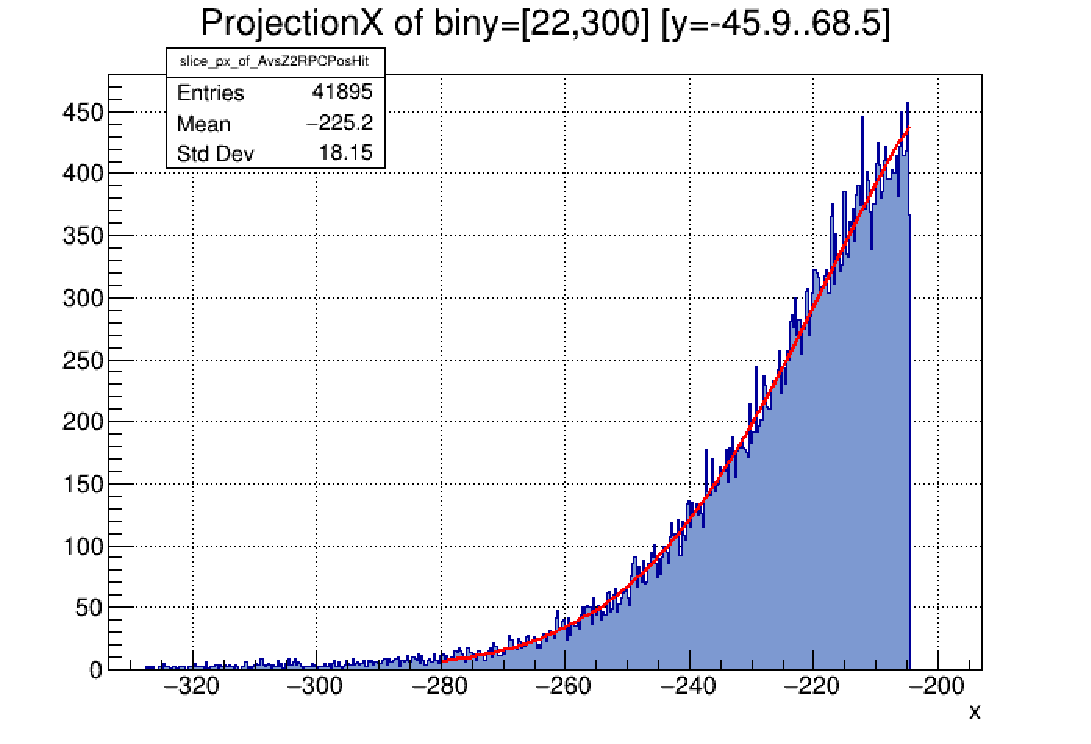
\includegraphics[width=0.7\textwidth]{Appendix/HitXProj}
	\caption[X projection of RPC hit map for $A/Q=2$ fragments]{Projection of the \gls{RPC} hit map for $A/Q=2$ fragments onto the $x$-axis, fitted with a Gaussian distribution. The fit yields a mean of $-185$~cm (relative to the $0^\circ$ line) and a standard deviation of 31.8 cm. From this distribution, it is estimated that approximately 26\% of the $A/Q=2$ fragments lie within the \gls{RPC} acceptance.}
	\label{fig:rpc_hitmap_xproj}
\end{figure}

These simulation studies provided a baseline expectation for the experiment, serving as a reference when interpreting the real data.
